\subsection{Solución actividad 3}

ACTIVIDAD 3. Respuesta al escalón de un sistema mecánico rotacional.\\
Dado el sistema de la figura 41:\\

1. ¿Cuál es la entrada y la salida del spinner?\\
La entrada es $\tau_{in}$, y la salida del spinner es la posición angular $\theta(t)$.\\ 


2. Si el modelo matemático del sistema es:\\
$$J\frac{d^2 \theta(t)}{dt^2} + B\frac{d\theta(t)}{dt} = \tau_{in}$$
donde J=2,B=0.2 y el torque de entrada $\tau_{in}$ es como se muestra en la figura 42.\\
De acuerdo a la ecuación anterior, tenemos que:
$$J\frac{d^2 \theta(t)}{dt^2} + B\frac{d\theta(t)}{dt} = \tau_{in}$$
$$\frac{d^2 \theta(t)}{dt^2} + \frac{B}{J}\frac{d\theta(t)}{dt} = \frac{1}{J}\tau_{in}$$
$$\frac{d^2 \theta(t)}{dt^2} = \frac{1}{J}\tau_{in} - \frac{B}{J}\frac{d\theta(t)}{dt}$$
Simulación del modelo matemático en SIMULINK:\\


\begin{center}
	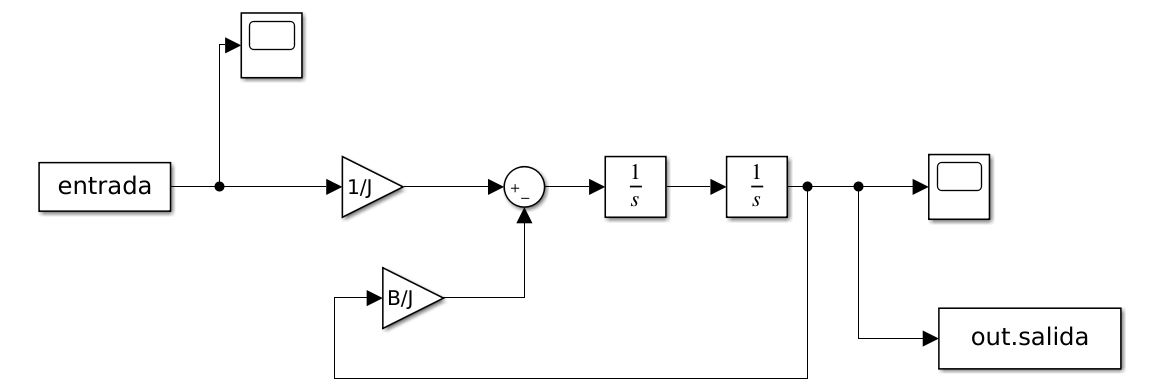
\includegraphics[scale=0.4]{ej3_1}
\end{center}



3. Obtenga la respuesta del sistema con ayuda de software especializado (anexar gráficas al final de la práctica).\\
Entrada de la simulación:\\
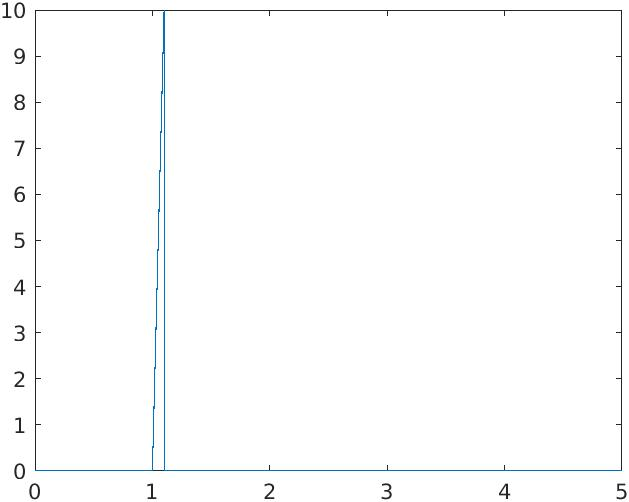
\includegraphics[scale=0.4]{EN} \\\\
Salida de la simulación::\\

\begin{center}
	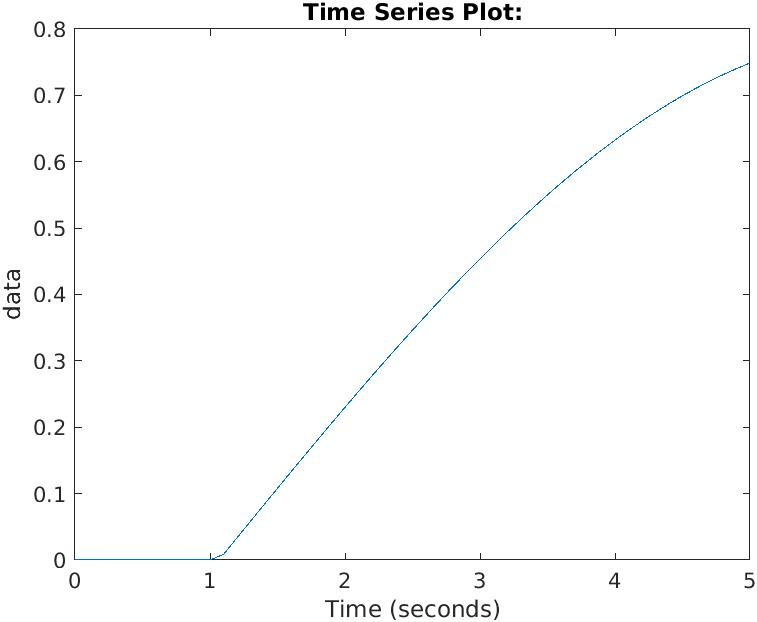
\includegraphics[scale=0.33]{Sal_ej3}
\end{center}



4. ¿Qué parámetros modificaría en el sistema para que gire por un tiempo más prolongado? Justifique matemáticamente su respuesta.\\
B(Coeficiente de fricción) y m(masa). Aunque también depende de la fuerza de entrada al sistema.